\subsection{Mapa cooperativo}
Mari0 es un juego opensource desarrollado por la comunidad. Este juego obtuvo mucha popularidad en los años 2012 a 2015. Durante esta epoca se creo un foro sobre el juego donde cualquier diseñador interesado podía enviar una copia de su mapa para que el resto de los jugadores del juego pudieran valorarlo. El juego ya trae varios mapas creados por los creadores del juego. Todos estos mapas pueden jugarse con más de 1 jugador, pero solo es necesario 1 jugador para completarlos. Aún así, ninguno de estos es estaba completamente diseñado para un minimo 2 o más jugadores.

En nuestro caso es necesario un mapa diseñado para 2 jugadores como minimo. Por ello teniamos 2 opciones. La primera opcion consistía en implementar el mapa nosotros mismos. Esta tarea no es demasiado dificil ya que el juego trae consigo un editor de niveles muy intuitivo y facil de usar. Aún así, esta tarea no estaba prevista y aún ser sencilla, es necesario un tiempo para desarrollar y testear el mapa. La otra opcion consistia en realizar una busqueda por el foro \cite{mari0-forum} con el objetivo de encontrar algún mapa que cumpliera estas características. 

Decidimos buscar en el foro y en caso de encontrar un mapa, analizar si era viable usarlo como el mapa pricipal del entorno. En caso de no encontrar ninguno viable, habría que implementarlo desde 0. Para facilitar la busqueda, se contacto con el usuario HugoBDesigner, un diseñador muy popular de mapas de Mari0, ya que este se dedicaba a realizar valoraciónes de los mapas que le enviaban otros usuarios y colaboraba activamente con los creadores del videojuego. Este diseñador colaboró con la busqueda aportadonos enlaces a 3 mapas cooperativos que él había jugado durante la epoca del 2012. De estos 3 enlaces, solo 1 permanecía activo. Este mapa llamado Bowser Cooperative Testing Initiative fue el que usamos para como mapa principal para el entorno. El mapa puede descargarse de \cite {mari0-mapa} gracias al diseñador Pixel Worker. 

Para comprobar que el entorno no puede ser resuleto por un solo agente usaremos la figura \ref {fig:mapa} que es el principio del primer nivel del mapa.

\begin{figure}[ht]
    \centering
    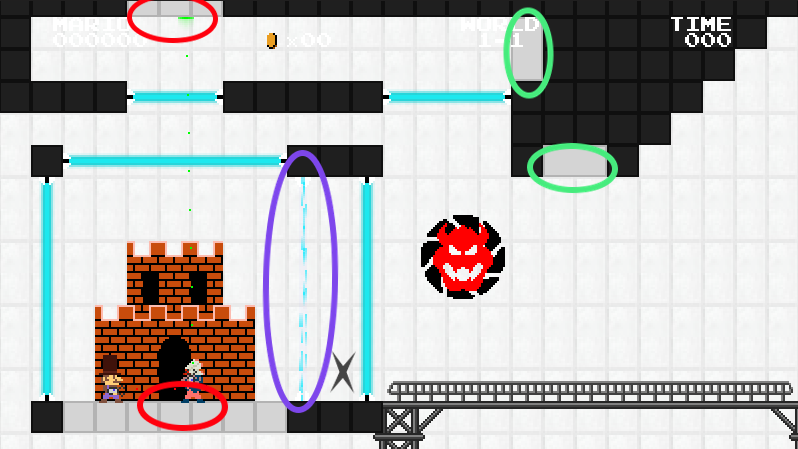
\includegraphics[width=0.9\textwidth]{img/mario-1-level.png}
    \caption{Nivel del mapa Bowser Cooperative Testing Initiative \cite {mari0-mapa}}
    \label{fig:mapa}
\end{figure}

La forma de resolver este nivel es la siguiente:
\begin{itemize}
    \item Paso 1: En primer lugar, uno de los dos jugadores, de ahora en adelante jugador 1, debe colocar un portal en cada uno de los circulos rojos indicados en la figura. Con este movimiento se consigue que el jugador 1 pase a la sección superior.
    \item Paso 2: El jugador 2 debe colocarse donde se encuentra la X indicada en la figura. Desde esta posicion debe disparar dos portales a los circulos verdes indicados en la figura. Con este paso el jugador 1, que se encuentra en la sección superior, será capaz de atravesar estos portales y pasar fuera del cuadrilatero inicial.
    \item Paso 3: Una vez el jugador 1 se encuentra fuera del cuadrialtero, el jugador 2 debera realizar las misma acciónes que el jugador 1 en el primer paso.
    \item Paso 4: Mientras eso ocurre, el jugador 1 deberá colocar sus portales donde los colocó el jugador 2 en el paso 2.
    \item Si se han realizado correctamente todos los pasos, ambos jugadores deberian haber salido del cuadrialtero inicial.
\end{itemize}

Es facilmente visible que un solo jugador no puede completar este primer nivel. Esto se debe a que desde la sección superior es imposible colocar los portales donde debe para salir del cuadrilatero. El resto de niveles del mapa incluyen este tipo de puzles los cuales, al igual que este, necesitan como minimo 2 agentes para ser resueltos.